\documentclass[11pt]{article}
\usepackage[T1]{fontenc}
\usepackage[latin1]{inputenc}
\usepackage{lmodern}
\usepackage{xcolor}
\usepackage{tikz,graphics,color,fullpage,float,epsf,caption,subcaption,tabularx, hyperref}
\usepackage{wallpaper}



\usepackage[margin=1in]{geometry}

\begin{document}
  \begin{titlepage}
    \centering
    \vspace*{11\baselineskip}
    \large
    \bfseries
    {\LARGE Pack Manager}\\[5\baselineskip]
    \normalfont
    \small
    CS130: Software Development\\
    Computer Science Department\\
    University of California, Los Angeles\\
    Spring 2015\\
    Git repository: \texttt{https://github.com/asanciangco/PackManager} \\[5\baselineskip]

    
\includegraphics[width=150pt]{img/pacman.png}
    \vfill
    {\large
	Alex Sanciangco\\
	Nick Westman\\
	Steven Holtzen\\
	Mitchell Binning\\
	Kacey Ryan\\
	Heather Blockhus\\}
  \end{titlepage}

\tableofcontents
\newpage

\section{Introduction and Motivation}
Pack Manager is a tool for helping you pack. It gives you a wardrobe list based on the weather of where you're going. It takes your (1) location, (2) time of travel, (3) personal dressing preferences, and gives you a set of clothes for you to wear and necessities that you can't forget. The goal is to make packing for an outing simple and fast. The application will have a very clean user interface; since its function is simple, its use must be equally simple. The application must be extensible, which means that adding new features must be a well-defined process that is easy.

\subsection{User Benefits}
A user may benefit from using our application if they are frequent travelers. It is very difficult to track what to bring when traveling, especially if travel arrangements frequently change or users travel to many locations in sequence. Our application can update them on changing weather patterns for arbitrarily complex trips spanning many days and destinations. 

Another example is someone traveling to an area with unfamiliar weather patterns. This makes it difficult to predict what would be necessary to bring. This user would simply enter their information into our application, which would automatically keep them up to date regardless of whether or not they know about monsoon season in Indonesia.

\section{Feature Overview} % this could use beefing up
    When the user first starts the application, he or she will be presented with a login screen where they can choose to log in with Facebook. Once logged in, the user will enter their preferences, at which point the application is ready to make packing suggestions. Once this initial login is complete, the preferences will be assigned to their account, making future trip planning seamless. A packing list is suggested after the user enters their destination, which can include multiple stops, date of departure, duration, and takes into account preferences and trip parameters. From the ``My Trips'' tab, the user can view and modify this packing list. The application will notify the user in case of weather changes; this will require updates to the packing list.

    \subsection{Initial Requirements}
        The following are the requirements that we initially set out to fulfill. 
        \subsubsection{General Requirements (G)}
        \begin{enumerate}
        \item Able to pull relevant weather information from Open Weather Map for
        arbitrary dates. (Related: G2, G4, G6, API1, API3, API4, UX7, UX8)

        \begin{enumerate}
        \item If no projected weather data, pull historical.
        \end{enumerate}
        \item Provide a framework for accepting and using user preferences. (Related:
        G5, G8)

        \begin{enumerate}
        \item User preferences must be consistent between sessions. 
        \item Must be able to export preferences. 
        \item Plan for eventual transition to decentralized storage (move to cloud).
        \end{enumerate}
        \item Create packing lists for vacations of arbitrary durations. (Related:
        G7)
        \item Provide a framework for trip preferences. (Related: G2, UX2)

        \begin{enumerate}
        \item Availability of laundry machines Level of cleanliness (\textquotedblleft I
        don\textquoteright t care about wearing underwear 13 times\textquotedblright ) 
        \item Specific activities Purpose (business, leisure, etc.) 
        \item These options affect the packing lists but are optional with customizable
        defaults.
        \end{enumerate}
        \item Sends user a push notification if weather changes in destination will
        affect packing list, or a critical weather alert is issued. (Related:
        G1, API4)
        \item Ability to modify already created packing list. (Related: G4, G8)

        \begin{enumerate}
        \item Add items, remove items, reevaluate (pull weather again) 
        \end{enumerate}
        \item Ability to create an itemized list of clothing and other essentials
        for travel. (Related: G2, G7, UX1, UX4, UX6, API2)

        \begin{enumerate}
        \item List can be customized after suggestion by user.
        \end{enumerate}
        \item Allow the user to login through Facebook. (Related: API3, API6)
        \end{enumerate}
        \subsubsection{User Experience (UX)}
        User Experience:
        \begin{enumerate}
        \item 3 user input (minimum) to get to a packing list: start date, duration,
        location. (Related: G5, G8)

        \begin{enumerate}
        \item Additional options available if necessary
        \item Duration must be nonnegative
        \item Destination: zip code or city, state/country
        \end{enumerate}
        \item Prompt for user preferences on first launch. (Related: G3, G5)
        \item Obtain user feedback after a trip to adjust user temperature preferences.
        (Related: API4)
        \item User can store packing lists upon save (Related: G8, UX5, API2)

        \begin{enumerate}
        \item Possibly autosave
        \end{enumerate}
        \item Export lists to other apps (reminders, calendar) (Related: UX4)
        \item Packing lists formatted as a table. Each row composed of item and
        quantity (e.g. T-Shirt x3, Socks x4, Suntan Lotion x1, Umbrella x1)
        (Related: G8)
        \item Error Reporting: If network unavailable, prompt user for solution
        (Related: API1, API4, G1)
        \item Error Reporting: No relevant weather information for provided destination
        (Related: API1, API4)
        \end{enumerate}
        \subsubsection{API Interactions and Extensibility (API)}
        \begin{enumerate}
        \item Application has a single point of failure for interacting with external
        APIs (Related: G1, API3, API6)
        \item Packing and destination information can be exported in JSON format
        (Related: G8, UX4)
        \item Build a wrapper around Open Weather API and Facebook for easy API
        usage (Related: G1, G9, API1)
        \item Build a push notification framework for communicating with users in
        a device-agnostic way (Related: G6)
        \item The system must have the capability to be localized (allow for arbitrary
        languages and character sets to be used)
        \item Facebook API is used for login and identity management. (Related:
        G9, API1)
        \end{enumerate}

        \subsubsection{Non-Functional Requirements (NF)}
        \begin{enumerate}
        \item Test coverage and automated building 
        \item Free to download 
        \item Secure 

        \begin{enumerate}
        \item user cannot see your packing lists 
        \item Outside users cannot modify your packing lists through any API 
        \end{enumerate}
        \item iOS Application targeted for iOS 8 and above \end{enumerate}

    \subsection{Requirements Revisions}
    We added several new features that were not initially listed in our design requirements. We added the ability to autocomplete your location using the Google API. We also added a Google Maps visualization, so that users can see their destinations. These features were deemed necessary because it is necessary for a good user experience: without seeing on a map what you typed in, it might be the wrong location. It is also very hard to type in an exact address, so the autocomplete is necessary as well.

    We decided to omit some of the requirements that were less important. We decided not to export user data to other applications such as calendar and reminders because as we were designing our application we realized that i) exporting to the calendars app wouldn't be particularly useful, and ii) we would rather have the to-do list features of the reminders app remain within our app. We also realized that we didn't want to prompt users for the preferences on the initial launch of the application since this made for an obtrusive and confusing UX; we would rather get the users right into the functionality immediately, then allow them to change settings if they so desired. We decided against gathering user feedback after their trips also for UX reasons: we realized that users likely wouldn't open our application immediately after a trip since our app is intended to be used before a trip. Our application does not currently export packing information to JSON because at this time it is not necessary. However, the data structure that stores the packing list can easily exported to JSON if that functionality ever become relevant. Lastly, we did not end up implementing push notifications because that would require usage of Apple Push Notification Service (APNS), which would require us to develop a server to send the notifications.


\section{Design}
    The application is structured using the model-view-controller architecture dictated by the iOS development framework. In an iOS application, the overall flow is defined in storyboards. These files define transitions between panes, hold content. The main storyboards for our application is in the \texttt{Main\_iPhone.storypad} file. The storyboards are the views in this framework.

    The controllers can be found in the \texttt{Controllers} subdirectory. These files dictate the flow of control within the application; they are the glue between the storyboards and the models, which define how data is stored and manipulated. By carefully separating the concerns between storing and loading data from the user interface logic, we get a clean modular structure that allowed Heather and Alex to both work simultaneously on different aspects of the application. 



    \subsection{External API Usage}
    \subsubsection{Weather API}
    The Weather API is an important and very tricky component of our application. See \texttt{PackManager/WeatherAPI.m} for our implementation. We currently use Open Weather Map\footnote{See \texttt{http://openweathermap.org/}} in order to gather weather data, which gives us a 16 day weather forecast for a particular geographic coordinate. We also use the NOAA weather API\footnote{See \texttt{http://www.weather.gov/}} for date ranges that are outside of a 16-day weather forecast. This data source includes historical data and can allow us to make coarse-grained projections over a much greater timespan and in a larger area. However, we can not get historical weather API for out of the country, since the NOAA is a U.S. government organization. Both data sources have completely different output formats (which is why our parsing file is over 500 lines long!).

    \subsubsection{Google Places API}
    We used the Google Places API\footnote{See \texttt{https://developers.google.com/places/}} for auto-completion as the user is entering their desired destinations. Handling this API was tricky, since it has a limited number of requests per day. See \texttt{PackManager/GooglePlacesAPI.m} for implementation.


    \subsection{Class Diagrams}
    See Fig.\ref{fig:tripclass}, Fig.\ref{fig:packable}, Fig.\ref{fig:weather-api} for an overview of our class design decisions. 

    \begin{figure}
        \centering
        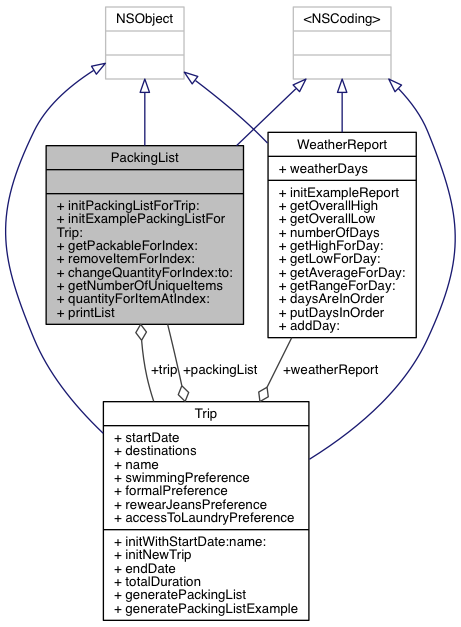
\includegraphics[scale=0.75]{img/trip_inheritance.png}
        \caption{The \texttt{Trip} class is the core structure for holding details related to an individual trip. Currently trip attributes are stored as booleans within this structure; we have plans to make these easier to change in the future.}
        \label{fig:tripclass}
    \end{figure}

    \begin{figure}
        \centering
        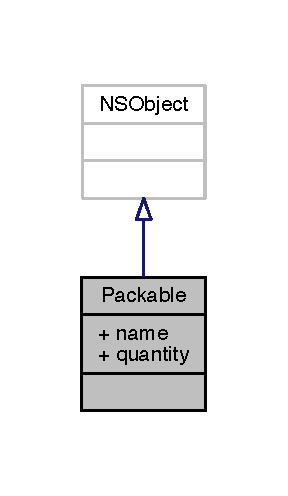
\includegraphics[scale=0.75]{img/packable.pdf}
        \caption{The packable interface defines the basic methods that are necessary to make an individual object packable. All articles of clothing will inherit this interface; it will likely need to be expanded as more required functionality is discovered.}
        \label{fig:packable}
    \end{figure}

    \begin{figure}
        \centering
        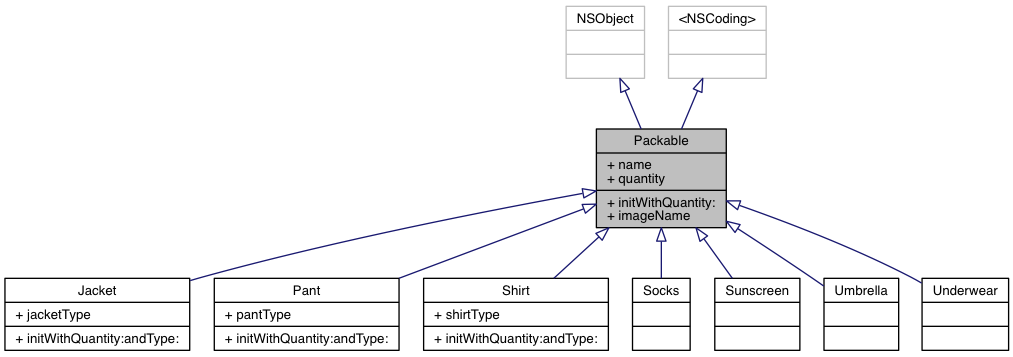
\includegraphics[width=\textwidth]{img/interface_packable.png}
        \caption{Packing lists are made up of packables and this diagram shows the packable class and the multiple types of packable items.}
        \label{fig:packable-interface}
    \end{figure}

    \begin{figure}
        \centering
        \begin{subfigure}[t]{0.45\textwidth}
            \centering
            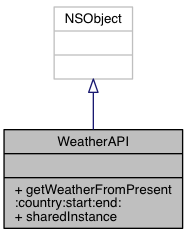
\includegraphics[width=0.5\textwidth]{img/interface_weather_api.png}
        \end{subfigure}%
        ~ 
        \begin{subfigure}[t]{0.45\textwidth} 
            \centering
            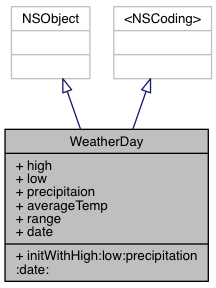
\includegraphics[width=0.7\textwidth]{img/interface_weather_day.png}
        \end{subfigure}
        \caption{As shown in the first figure, the trip takes into account the weather report, which is generated by the Weather API shown above. Additionally the weather report consists of weather days, shown above.}
        \label{fig:weather-api}
    \end{figure}

    \subsection{Clothes Selection Algorithm}
    In order to generate a list of items one should bring on their trip we needed to come up with an algorithm. The packing algorithm would have to account for the trip's duration, each day's weather, and a number of user preferences (i.e. re-wearing jeans, access to laundry, their hot cold preferences, etc). Our algorithm first initializes a packing list, checks each day's weather and appropriately increments clothing, and finally produces estimates based on user preferences. The initialization creates a packing list that contains the bare essentials such as toiletries. Additionally, the initialization will check if the user has marked if they will be swimming or need formal attire. If they checked swimming then it will include swimwear as a function of days. Next, for each day in the trip the algorithm calls several incrementing functions, one for each type of clothing (tops, bottoms, etc). Each of these incrementing functions have a simple interface that hides its implementation details from its caller, exercising the information hiding principle. Each function checks the day's average temperature against the user's temperature preference and perform different clothing increments based on what the user thinks of that day weather (hot, warm, normal, cool, cold). Finally, now that the algorithm has produced a maximal list, it checks the user's preferences for things like access to laundry and rewearable jeans and reduces the list's numbers. For example, if laundry is checked it will cap the max number for each type of clothing article. Similarly, re-wearing jeans would cap just the bottoms category. x

    \subsection{API Description}
    Our API description can be found inside of our documentation, in \texttt{doc/html/index.html}. We took care to document most of our classes and functions in the Doxygen style, allowing for automatically generated formatted descriptions. An example of our documentation can be found in Fig.\ref{fig:doc}. Overall, all API accesses flow through the \texttt{WeatherAPI} and \texttt{GoogleAPI} classes; these classes act as mediators, filtering information and handling de-bouncing of frequent requests. 

    \begin{figure}
    \centering
    
\includegraphics[scale=0.5]{img/doxygen.png}
    \caption{Example of the documentation generated by Doxygen for the \texttt{WeatherAPI} class.}
    \label{fig:doc}
    \end{figure}




\section{Quality Assurance}

\subsection{Testing}
We set up a test harness using Travis CI\footnote{See \texttt{https://travis-ci.org/}}. Travis CI is a continuous integration suite that automatically runs our tests whenever a pull request is performed on Github. Before a change is merged all the tests are run in order to guarantee that all code that gets checked in passes all the tests. See Fig.\ref{fig:travis} for an example Travis CI output.

Travis CI configured in the \texttt{.travis.yml} file, which specifies the language framework as well as the test harness. Our tests can be found in the \texttt{PackManagerTests} directory. We used Nocilla\footnote{See \texttt{https://github.com/luisobo/Nocilla}} in order to create mock HTTP requests to simulate the weather API behavior. This lets us test the Weather API without making HTTP calls. We then use these same mock API calls throughout the rest of our tests. We test much of our application in isolation of the Internet, which allows our tests to be reproducible with expected outcomes, letting us use assertions.

We used testing in order to validate our application; the goal is not to achieve ultra high reliability, since our application is likely to rapidly change. In line with this goal, we have isolated unit tests for the core functionality, including tests for the weather API, Google APIs, the packing algorithm, and the integration between these components. These tests can be found in \texttt{PackManagerTests}. 

We make extensive use of swizzling, which is a built-in utility for iOS that lets us swap out implementations of individual methods for stub methods. For example, when the \texttt{getDate} method is called, we return a specific date for use in assertions (for example, Jan. 1 1970). This lets us make assertions regardless of what day of the week it is.



 
\begin{figure} 
\centering
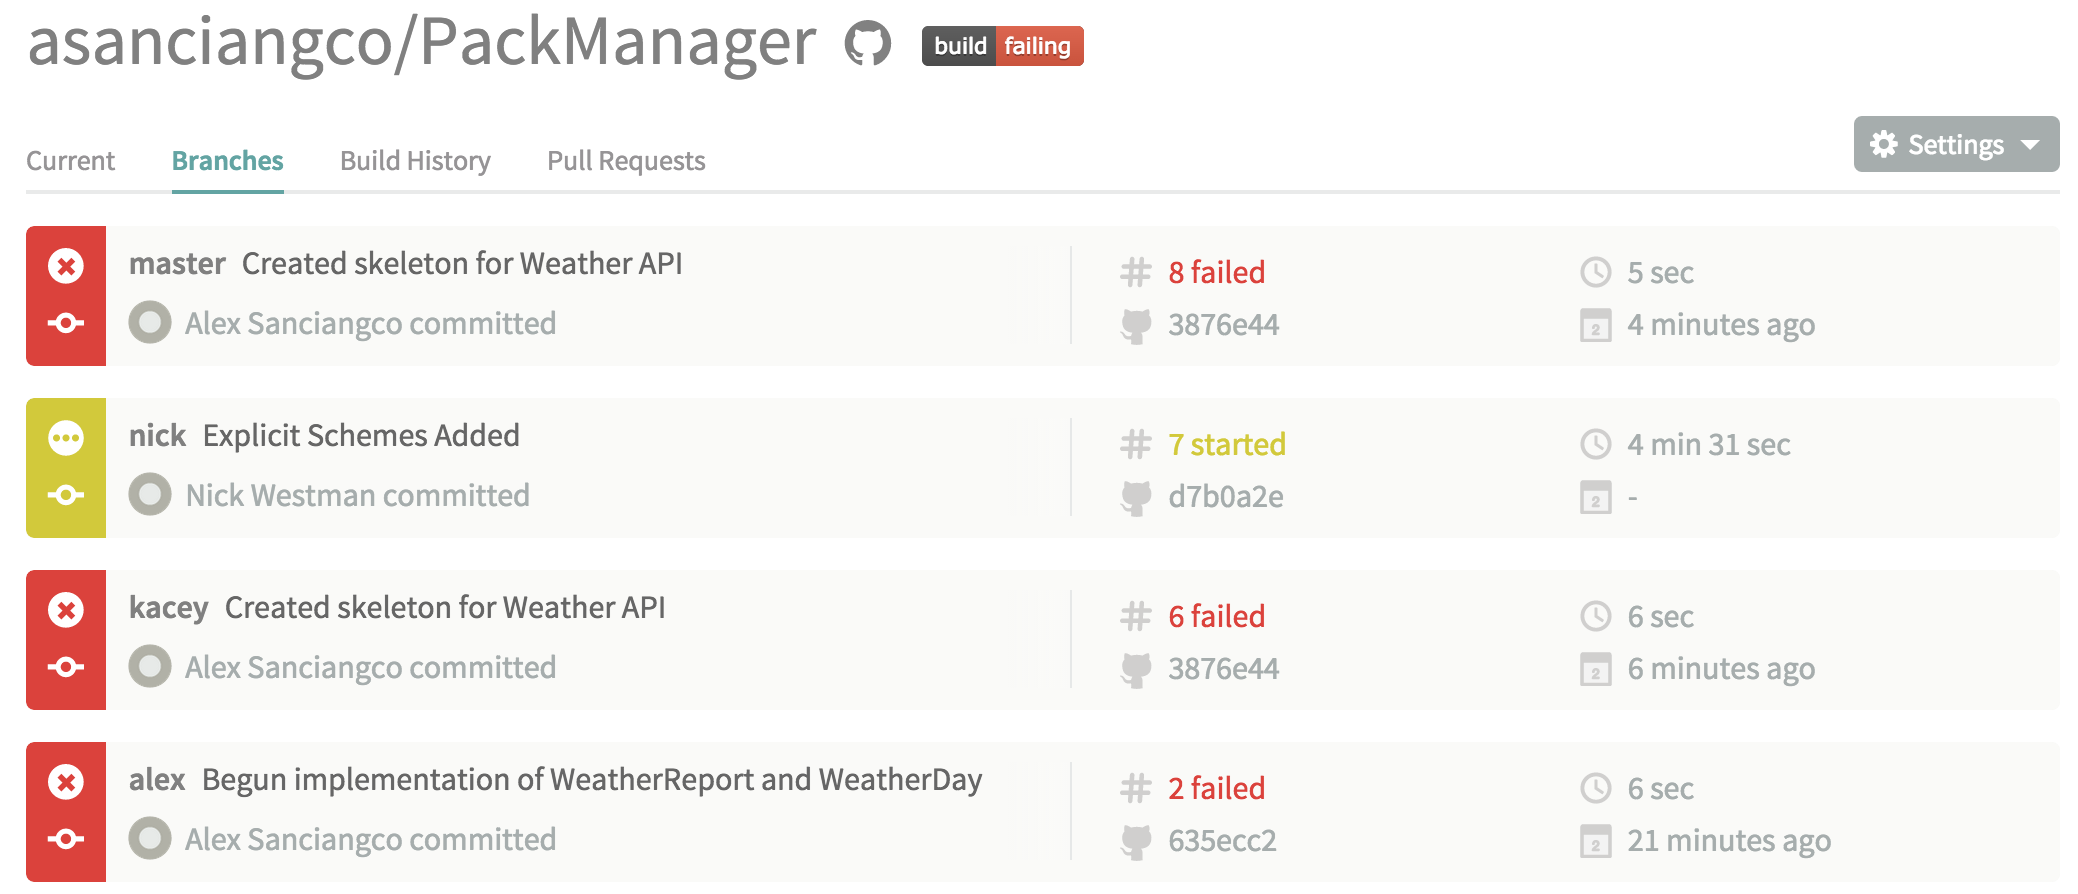
\includegraphics[width=\linewidth]{img/travis.png}
\caption{Output of Travis CI. It shows the status of all branches as well as whether or not they are currently passing the tests that are specified in \texttt{.travis.yml}. This will prevent ever merging a branch that does not pass tests, which will prevent regressions.}
\label{fig:travis}
\end{figure}

\section{User Interface}
See Fig.\ref{fig:ui} for some screen shots of the user interface.

\begin{figure}
    \centering
    \begin{tabular}{ccc}
    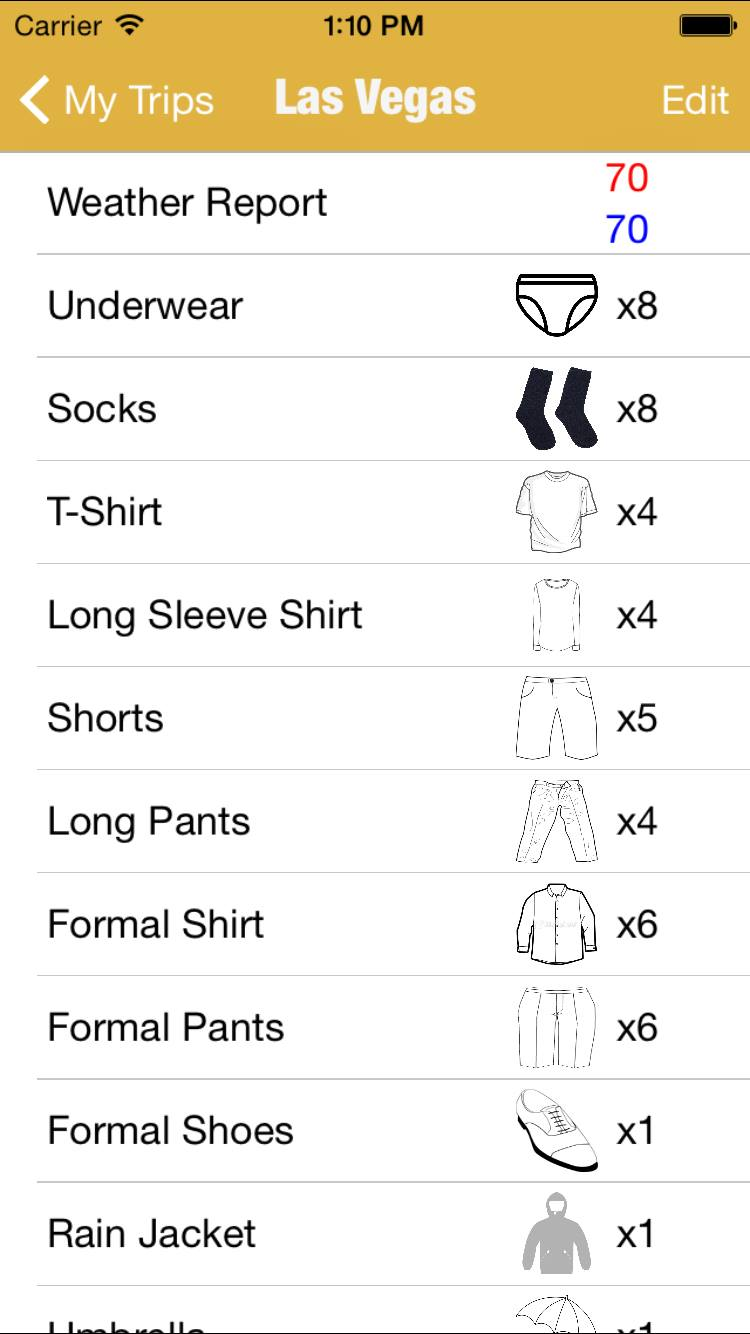
\includegraphics[scale=0.2]{img/ui-2.jpg} & 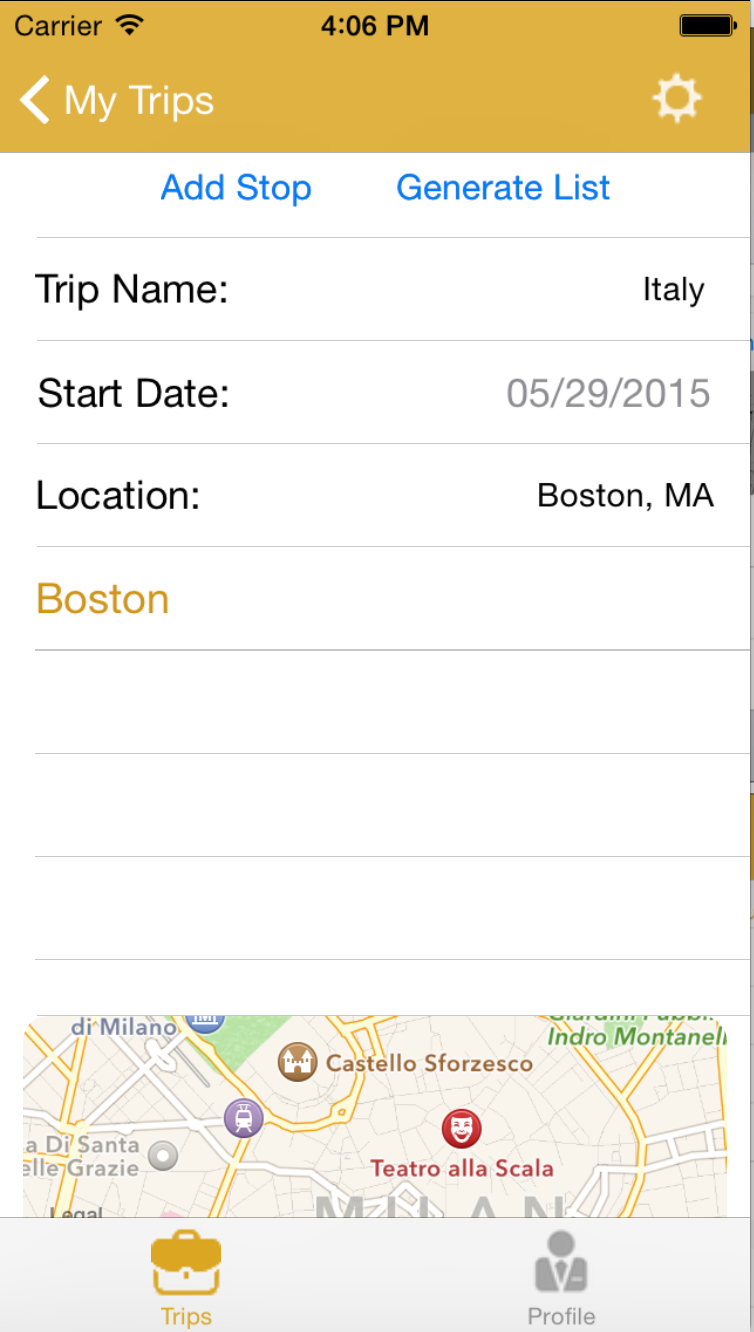
\includegraphics[width=151pt]{img/ui-8.png} & 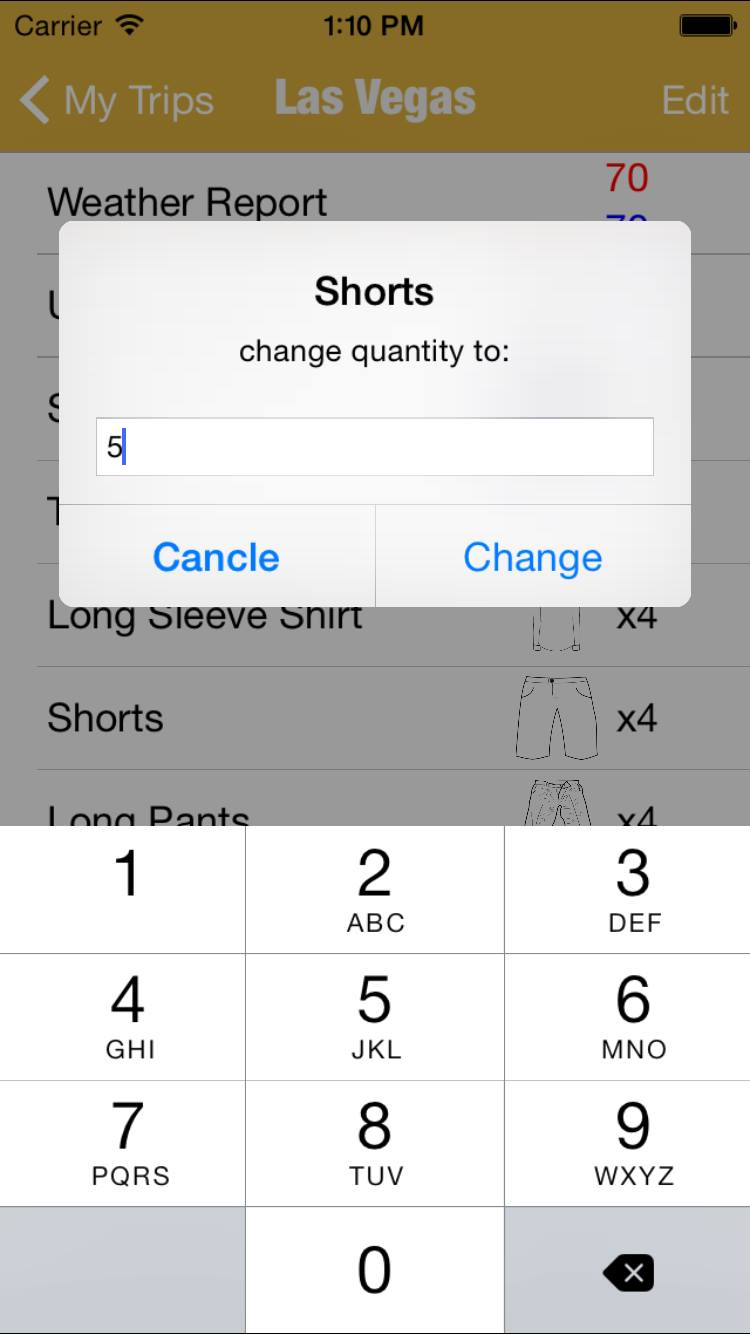
\includegraphics[scale=0.2]{img/ui-7.jpg}\\
    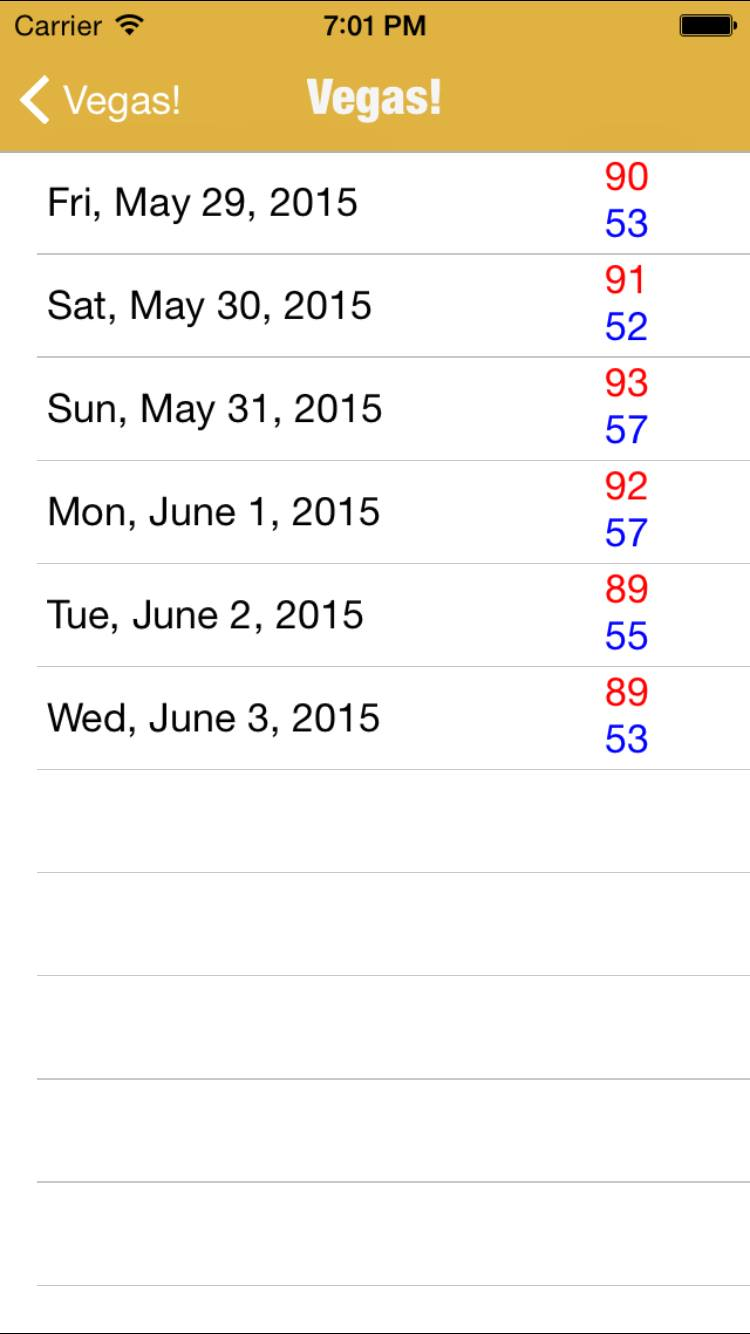
\includegraphics[scale=0.2]{img/ui-5.jpg} & 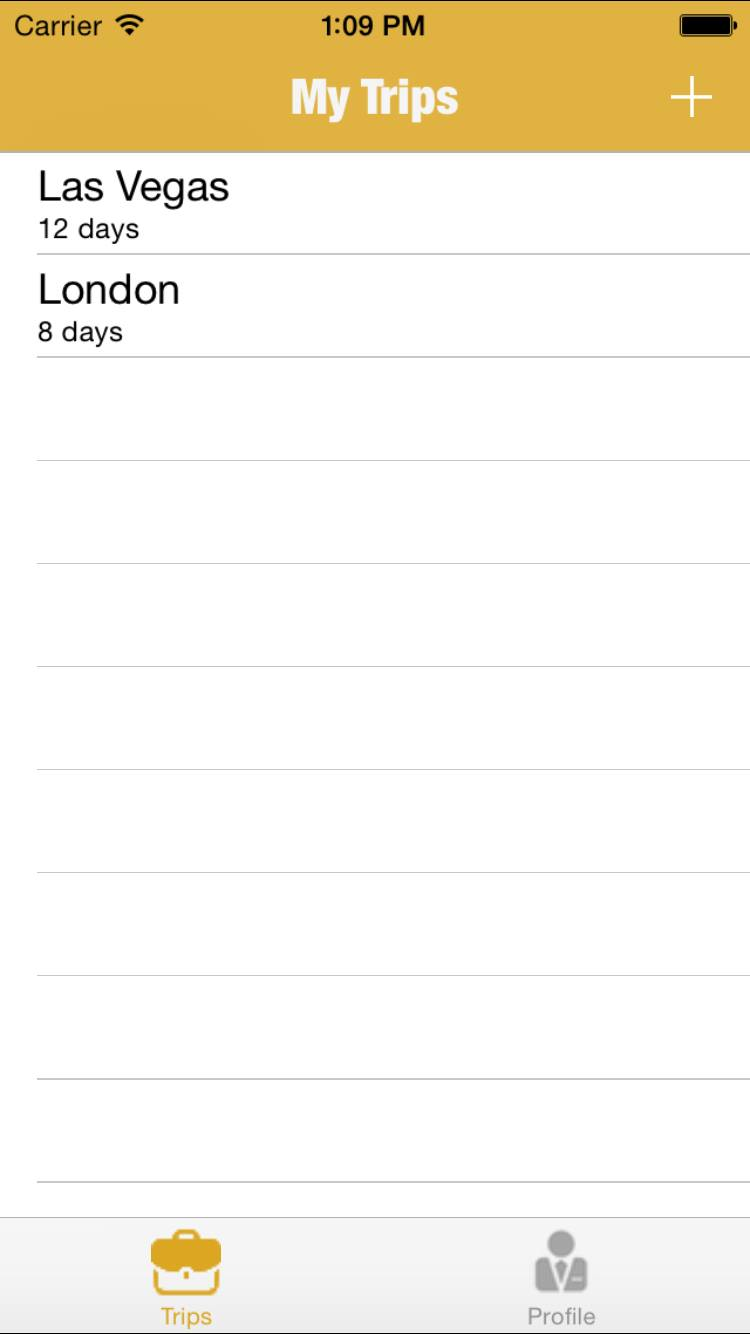
\includegraphics[scale=0.2]{img/ui-6.jpg} & 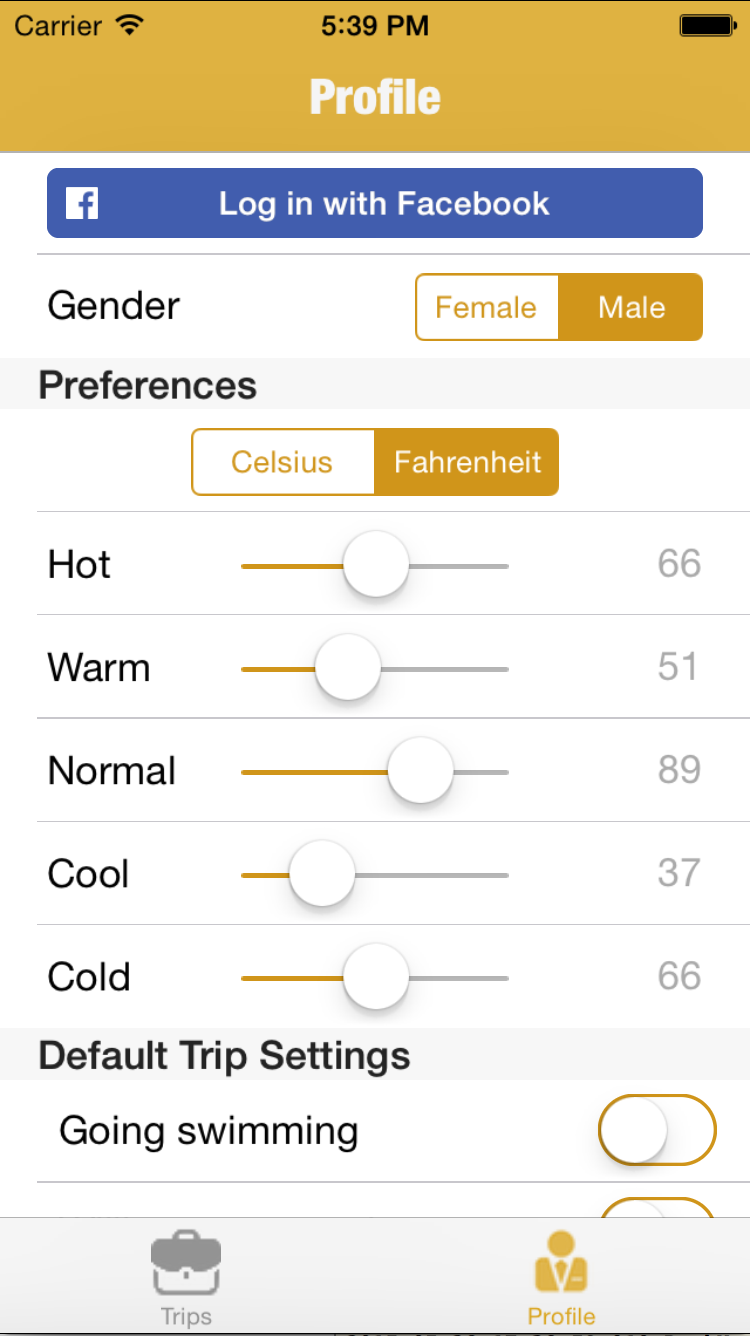
\includegraphics[width=151pt]{img/ui-4.png}
    \end{tabular}
    \caption{User interface snapshots. Top left, a generated packing list; top middle, the trip creation screen with location auto-complete and Google maps visualization; top right, an option to enter a specific number of shorts; bottom left, example weather forecast for a trip; bottom middle, selecting between multiple pre-made trips; bottom right, the user profile, with Facebook login.}
    \label{fig:ui}
\end{figure}

% added autocompleting forms
% display map based on where you are going to go
% 

\section{Contributions}
\begin{enumerate}
\item Heather worked on the user interface. She worked on developing flow of the application, working closely with Alex. Heather is experienced with designing user interfaces for iOS.
\item Alex is the lead programmer. He worked on integrating Heather's user interface with Kacey's weather API, as well as being a source of knowledge on general iOS development and Objective-C, which many group members were not familiar with.
\item Steven worked on writing the report and the documentation. He added Doxygen and used \LaTeX  to write the paper. 
\item Kacey worked on the weather API, doing research and wrapping it to make it accessible and easy to use. 
\item Mitchell worked on the presentation and report as well as general programming tasks.
\item Nick was in charge of build management and testing, integrating Travis-CI and managing the test infrastructure.
\end{enumerate}

\section{Conclusion}
We completed almost all of the requirements that we listed for our application on time, in addition to some extra requirements that we felt were necessary as we were developing. In total the project is over 3000 lines of Objective-C and over 1300 lines of comments, with major commits and contributions from every group member, even the ones that were not initially familiar with Objective-C. 

\end{document}